\documentclass[conference]{IEEEtran}
\usepackage{multirow}
\usepackage{subfigure}
\usepackage{graphicx}
\usepackage{graphics}
\usepackage{rotating}
\usepackage{verbatim}
\ifCLASSINFOpdf
\else
\fi
\hyphenation{op-tical net-works semi-conduc-tor}
\begin{document}
\title{Dirt Spot Sweeping Random Strategy}
\author{\IEEEauthorblockN{Mian Asbat}
\IEEEauthorblockA{Department of Computer Science\\
University of York\\
York, United Kingdom\\
Email: mian.ahmad@york.ac.uk}

\and
\IEEEauthorblockN{Manuel Oriol}
\IEEEauthorblockA{ABB Corporate Research\\
Industrial Software Systems\\
Baden-Dattwil, Switzerland\\
Email: manuel.oriol@ch.abb.com}}

\maketitle

%%%%%%%%%%%%%%%%%    ABSTRACT   %%%%%%%%%%%%%%%%%%%%
\begin{abstract}
This paper presents an enhanced and improved form of automated random testing, called Dirt Spot Sweeping Random (DSSR) strategy. DSSR strategy is a new strategy that combines ordinary random strategy and random plus strategy to achieve their combined benefits and additionally sweeps the dirt spots (Faulty patterns) in the program code for faults. It is based on two intuitions, first is that test values in boundaries of equivalence partition are interesting, using these test values in isolation can detect new faults in the system with fewer number of test executions, which produce high impact on test results while second is that faults reside in block and strip patterns inside the input domain therefore when a fault is found, using neighbouring values of the fault finding value can reveal more faults quickly which consequently increases the test performance.
\end{abstract}
\IEEEpeerreviewmaketitle



%%%%%%%%%%%%%%%%%    INTRODUCTION   %%%%%%%%%%%%%%%%%%%%
\section{Introduction}
All the strategies used in the automated software testing tools for finding faults in the given Software Under Test (SUT) aim to detect maximum number of faults in minimum amount of time. This can be achieved if test strategy selects more faults targeted test cases from the input domain for the given SUT, however, it is not that easy to produce such targeted test cases because each system has its own requirements and functionality.\\
\indent The researchers \cite{Chen2008} found that the performance of random testing can be increased by slightly altering the technique of test case selection. In adaptive random testing, Chen et al.  \cite{Chen2008} found that the performance of random testing increases by up to 50\% when test input is selected evenly which is spread across the whole input domain. Similarly Restricted Random Testing \cite{Chan2002}, Feedback directed Random Test Generation \cite{Pacheco2007a}, Mirror Adaptive Random Testing \cite{Chen2003} and Quasi Random Testing \cite{Chen2005} also stressed on the need of test case selection covering whole of the input domain for better results.\\
\indent To produce more relevant and fault targeted test data for random testing we developed an enhanced, more efficient technique called Dirt Spot Sweeping Random (DSSR) strategy.  Before its implementation, working and evaluation, the following research questions about the DSSR strategy were formulated and subsequently addressed:
\begin{enumerate}

\item To get highly efficient algorithm to cope with the combination of strategies including pure random, random plus and spot sweeping.

\item To get high number of unique faults because according to Chen et al. \cite{Chen2006} most of the faults reside in block and strip pattern which is efficiently covered by DSSR strategy. 

\item To get  low number of unique faults and high number of similar faults because the faults in the same block and strip pattern across the program might be of similar nature.

\item  Not to get any particular improvement if the program don't contain any block or strip pattern but contain only point pattern.

\item  DSSR strategy might consume more time to execute the same set of test cases than random and random plus strategy because of extra processing when analysing values at runtime, transferring them to the list of interesting values and selecting appropriate test value from the list when required during test.

\end{enumerate}
The rest of this paper is organised as follows. The sections, II to X, describe Dirt Spot Sweeping Random strategy, Implementation of DSSR strategy, Experimental setup and analysis, evaluation of DSSR strategy, Experimental results, Unique faults found by DSSR strategy, discussion, conclusion and future work respectively.



%%%%%%%%%%%%%%%%%    DIRT SPOT SWEEPING STRATEGY  %%%%%%%%%%%%%%%

\section{Dirt Spot Sweeping Random Strategy}
Dirt Spot Sweeping Random (DSSR) strategy is a new random test strategy developed during this study. DSSR strategy is the combination of two existing strategies i.e. pure random and random plus with the addition of one new strategy called spot sweeping. It is based on two intuitions. Intuition No. 1 is that boundaries have interesting values and using these values in isolation can provide high impact on test results, while intuition No. 2 is that faults can reside in block and strip pattern thus using neighbouring values of the fault finding value can lead us to the next fault in the same block or strip. This increases the performance of the test strategy in terms of executing fewer number of test cases with more number of faults. Each component is briefly explained as follows.

\subsection{Random Testing Strategy}
Random testing is a black-box testing technique in which the SUT is executed against randomly selected test data. Test results obtained are compared against the oracle defined using SUT specifications in the form of contracts or assertions. In the absence of contracts/assertions the exceptions defined by the programming language in which the program is developed is used as test oracle. According to Beizer, \cite{Beizer1990} software performance is directly dependant on the combination of two main factors that include correctness and robustness. Correctness is the expected behaviour of the software based on its specifications while robustness is the behaviour of the software which is not defined in its specifications. Since random testing generates test data randomly without any specific pattern therefore it effectively test the performance of software by evaluating it for both correctness and robustness. Because of its black-box testing nature it is particularly effective in testing softwares where the developers wants to keep the source code secret \cite{Chen2010}. The generation of random test data is comparatively cheap and does not require too much intellectual and computation efforts \cite{Ciupa2009}, \cite{Ciupa2008}. It is mainly for this reason that various researchers have recommended this strategy for incorporation in automatic testing tools \cite{Ciupa2008a}. YETI \cite{Oriol2010a}, \cite{Oriol2010}, AutoTest \cite{Leitner2007}, \cite{Ciupa2007}, QuickCheck \cite{Claessen2000}, Randoop \cite{Pacheco2007}, JArtage \cite{Oriat2004} are a few of the most common automated testing tools based on random strategy.\\
\indent In the past random testing went through some controversies in terms of performance. The efficiency of random testing was made suspicious with the intuitive statement of Myers \cite{Myers2004} who termed random testing as one of the poorest methods for software testing, however in science there is no substitute for experimental analysis and later on various experiments performed by different researchers \cite{Ciupa2007}, \cite{Duran1981}, \cite{Duran1984}, \cite{Hamlet1994} and \cite{Ntafos2001}  experimentally proved that random testing is simple to implement, cost effective, highly efficient and free from human bias compared to its rival techniques. 

\subsection{Random Plus Strategy}
Random plus strategy \cite{Leitner2007} is an updated version of the pure random strategy. It is a modified form of random strategy that uses some special pre-defined values which can be simple border values or values that have high tendency of finding faults in the SUT. Boundary values \cite{Beizer1990} are the values on the start and end of a particular type. For instance,  if input for a SUT is days of an year which is expressed in numbers from 1 to 365 then -2, -1, 0, 1, 2, 363, 364, 365, 366 367, can be considered as border values as shown in Figure \ref{fig:boundaryValues}. 

\begin{figure}[ht]
\centering
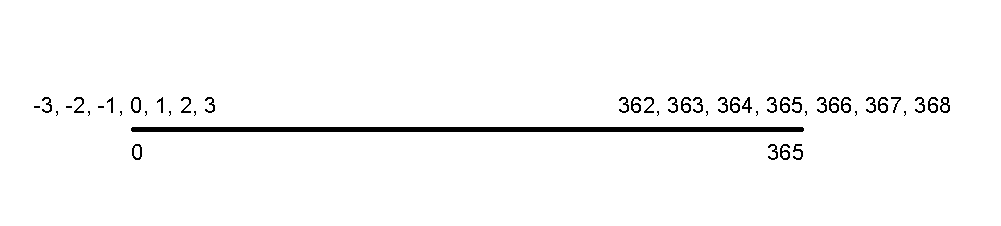
\includegraphics[width= 9cm,height=2cm]{boundary.png}
\caption{Boundary values for input domain from 0 to 365}
\label{fig:boundaryValues}
\end{figure}

Similarly the tester might also add some other special values that he consider effective in finding faults for the current SUT. For example, if a program under test has a loop from -50 to 50 then the tester can add -55 to -45, -5 to 5, 45 to 55 etc to the pre-defined list of special values in order to be selected for a test.This static list of interesting values is manually updated before the start of the test if require and has slightly high priority than selection of random values because of its more relevance and high chances of finding faults for the given SUT. It is found that these special values have high impact on the results particularly detecting problems in specifications \cite{Ciupa2008}.

\subsection{Dirt Spot Sweeping}
Chen et al. \cite{Chen2008} found that there are patterns of failure causing inputs across the input domain as shown in Figure \ref{fig:patterns}. They divided these patterns into three types called block, point and strip patterns. They also argued that a strategy can get more chances of hitting these fault patterns if test cases far away from each other are selected. Various other researchers \cite{Chan2002}, \cite{Chen2003} and \cite{Chen2005} also tried to generate test cases further away from one another targeting these patterns and achieved higher performance.\\
\begin{figure}[ht]                                    
\centering
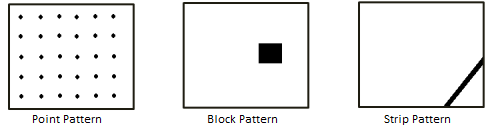
\includegraphics[width= 8cm,height=2.5cm]{ART_Patterns.png}
\caption{Failure patterns across input domain \cite{Chen2008}}
\label{fig:patterns}
\end{figure}

Spot sweeping is the part of the DSSR strategy that come in to action when a fault is found in the system. On finding fault, it immediately add the value causing the fault and its neighbouring values to the already existing list of interesting values at run time. For example in a program if an int value of 50 causes a fault then spot sweeping will add values from 45 to 55 to the list of interesting values. Now if that fault lays in the block or strip pattern then adding its neighbours will explore all the faults present in that strip. We can also say that in random plus the list of interesting values remain static/constant whereas in DSSR strategy the list of interesting values is dynamic and changes during the test execution of each program.\\

\begin{figure}[ht]
\centering
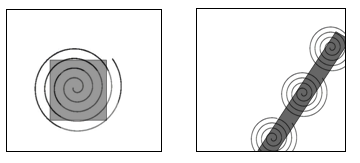
\includegraphics[width=8cm,height=2cm]{block2.png}
\caption{DSSR covering block and strip pattern}
\label{fig:block2}
\end{figure}

Figure \ref{fig:block2} shows how spot sweeping explores the faults residing in the block and strip patterns of a program. 

The faults coverage from the block and strip pattern is shown in spiral form because first fault will lead to second, second to third and will continue until it ends. But if that fault is positioned on the point pattern then the added values will not be very effective because point pattern is only an arbitrary fault point in the whole input domain.

\subsection{Structure of Dirt Spot Sweeping Random Strategy}

\hspace{10 mm}The DSSR strategy is explained with the help of flow-chart in Figure \ref{fig:Working_DSSS}. In this process the DSSR strategy continuously track the number of faults during the execution of the test session. To keep the system fast this tracking is done in a very effective way with 0 or minimum overhead \cite{Leitner2009}. Execution of test is performed normally until a fault is found in the SUT. When a fault is found the program not only copy the value that lead to the fault, but also copy its surrounding values to the variable list of interesting values. From the flow-chart you can see that if the fault finding value is of primitive type then the test strategy DSSR finds the type of that primitive value and add values only of that particular type to the interesting values list. Addition of these values increases the size of the list of interesting values which provide relevant test data for the remaining test session and the new generated test cases are more targeted towards finding new faults in the given SUT.\\
\begin{figure}[ht]
\centering
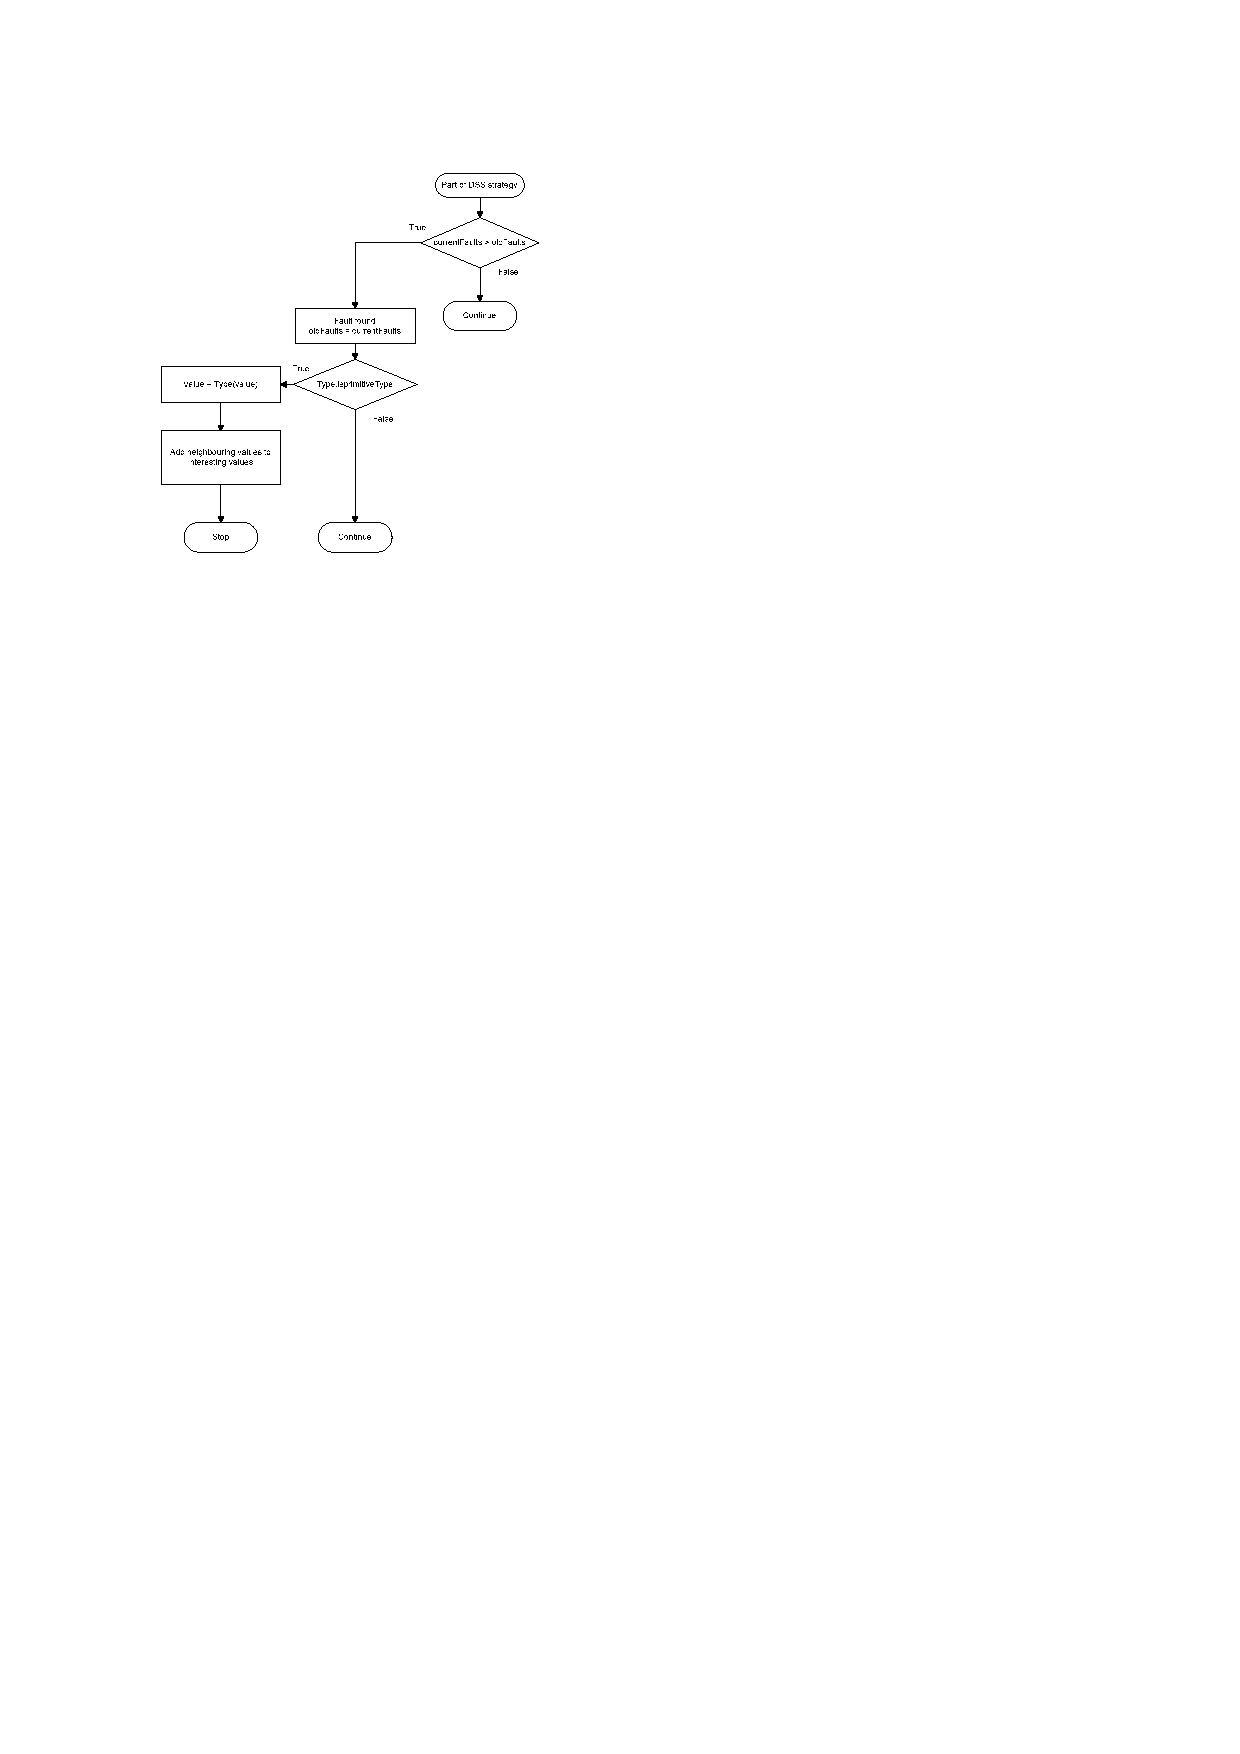
\includegraphics[width=8cm,height=9cm]{flowchart1.pdf}
\caption{Working mechanism of DSSR Strategy}
\label{fig:Working_DSSS}
\end{figure}

Border values and other special values that have high tendency of finding faults in the SUT are added to the list by random plus strategy (extension of pure random) prior to the start of test session where as to sweep the failure pattern, fault value and fault surrounding values are added at run time after a fault is found. Table \ref{table:addvalues} contain the values that are added to the list of interesting values when a fault is found. The test value is represented by X where X can be int, double, float, long, byte, short, char and String. All values are converted to their respective types before adding to the list of interesting values and vice versa.

\begin{table}[ht]
%\scriptsize
\caption{Neighbouring values for primitive types and String} % title of Table
\centering % used for centering table
\begin{tabular}{| l | l |} % centered columns (4 columns)
\hline\hline %inserts double horizontal lines
Type & Values to be added\\ [0.5ex] % inserts table
%heading
\hline % inserts single horizontal line
\multirow{1}{*}{X is int, double, float, } & ~ X,  X+1, X-1 \\ % inserting body of the
\multirow{1}{*}{long, byte, short \& char} &  \\ 

\hline
\multirow{8}{*}{X is String} & ~ X\\ % inserting body of the table

& ~ X + ``  "\\ % inserting body of the table
& ~ ``  " + X \\ % inserting body of the table
& ~ X.toUpperCase() \\
& ~ X.toLowerCase() \\
& ~ X.trim() \\
& ~ X.substring(2) \\
& ~ X.substring(1, X.length()-1) \\[1ex]
\hline
\hline %inserts single line
\end{tabular}
\label{table:addvalues} % is used to refer this table in the text
\end{table}
\subsection{Explanation of DSSR with an example program}
We explain the concept of DSSR through a simple program. The program is seeded with at least three faults. The first is division by zero exception denoted by 1 and others are in the form of assertion statements denoted by 2 and 3 in the following program.  Below we describe how DSSR strategy will perform execution when the following class is expose to testing.\\


\begingroup

    \fontsize{7pt}{8pt}\selectfont
    
\noindent
/\textasteriskcentered \textasteriskcentered \\*
\textasteriskcentered   ~ Calculate square of given number and verify results. \\*
\textasteriskcentered   ~ Code contain 3 faults.\\*
\textasteriskcentered   ~ @author (Mian and Manuel) \\* 
\textasteriskcentered   ~ @version (1.1, 11/07/12)\\*
\textasteriskcentered / \\*

\noindent public class Math1 \{\\
\indent public void calc (int num1) \{\\

\indent // Square num1 and store result.\\*
\indent int result1 = num1 * num1;\\*

%\indent \textbackslash\textbackslash Divide result1 by num1 and store result.\\*
\indent int result2 = result1 / num1;............................................................. Fault 1\\

%\indent \textbackslash\textbackslash To check that the revert of result is the received value.\\*
\indent assert Math.sqrt(result1) == num1;.................................................. Fault 2\\

%\indent \textbackslash\textbackslash To check that the value of result is positive.\\*
\indent assert result1 $>$= num1;................................................................... Fault 3\\
\indent \}  \\*
\noindent\}\\

\endgroup
In the above code one primitive variable of type ``int" is used, therefore, the input domain for DSSR is from -2,147,483,648 to 2,147,483,647. DSSR further select some values like 0, Integer.MIN\_VALUE and Integer.MAX\_VALUE as interesting values and increase its priority for selection as test values. 
When test start all 3 faults are quickly discovered by DSSR strategy in the following order.\\
\indent \textbf{Fault 1:} The DSSR strategy might select value 0 for variable ``num1"  in the first test case because 0 is available in the list of interesting values and therefore its priority for selection is higher than other values. This will cause Java to generate division by zero exception because any integer divided by zero is infinity.\\*
\indent \textbf{Fault 2:} When DSSR strategy catch the first fault it add the fault generated and its surrounding values to the list of interesting values which includes 0, 1, 2, 3 and -1, -2, -3 in this case. For second test case DSSR strategy may pick -3 as a test value and it will lead us to the second fault where assertion (2) will fail because the square root of 9 will be +3 instead of the original value -3.\\*
\indent \textbf{Fault 3:} Few tests later DSSR strategy may select Integer.MAX\_VALUE for variable ``num1" which is also available in the list of interesting values and it will lead us to the 3rd fault because result1 will not be able to store the square of Integer.MAX\_VALUE. Instead of the actual calculated square value Java will assign a negative value (Java language rule) to variable result1 which will again lead to the violation of next assertion (3).\\*
\indent From the above execution process we can understand that, in this example, pre-defined values including border values, fault finding values and its surrounding values lead us quickly to the available faults and in less number of tests as compared to Random and Random plus strategy which takes longer to discover the same faults because they try to find faults randomly even when the first fault found is very close to the second.


%%%%%%%%%%%%%%%%%    IMPLEMENTATION OF DSSR STRATEGY   %%%%%%%%%%%%


\section{Implementation of DSSR strategy}
Instead of reinventing the wheel the DSSR strategy is implemented in an existing open-source automated random testing tool called YETI \cite{Oriol2011}, \cite{Oriol2012}. YETI tool is developed in Java which is capable of testing systems developed in procedural, functional and object-oriented languages. Its language-agnostic meta model enables it to test programs written in multiple languages including Java, C\#, JML and .Net. The core features of YETI includes easy extensibility for future growth, speed of up to one million calls per minute on java code, real time logging, real time GUI support, ability to test programs using multiple strategies and auto generation of test report at the end of the test session. A number of hitherto faults have successfully been found by YETI in various production softwares. \\
\indent YETI can be divided into three main sections including core infrastructure, language-specific bindings and strategies. The core infrastructure represents routines, a group of types and a pool of specific type objects. The  language specific bindings contain the code to make the call and process the results. The strategies section defines the way to select the class/module to test random selection of routine/method from the given module and get instances of the required type during testing. Most common strategies in this section are random, random plus, DSSR strategy is also added to the strategies section of YETI tool with the class name YetiDSSRStrategy. It is extension of YetiRandomStrategy which in itself is extension of an abstract class YetiStrategy. The class hierarchy is shown in Figure \ref{fig:hierarchyofDSSR}.

\begin{figure}[ht]
\centering
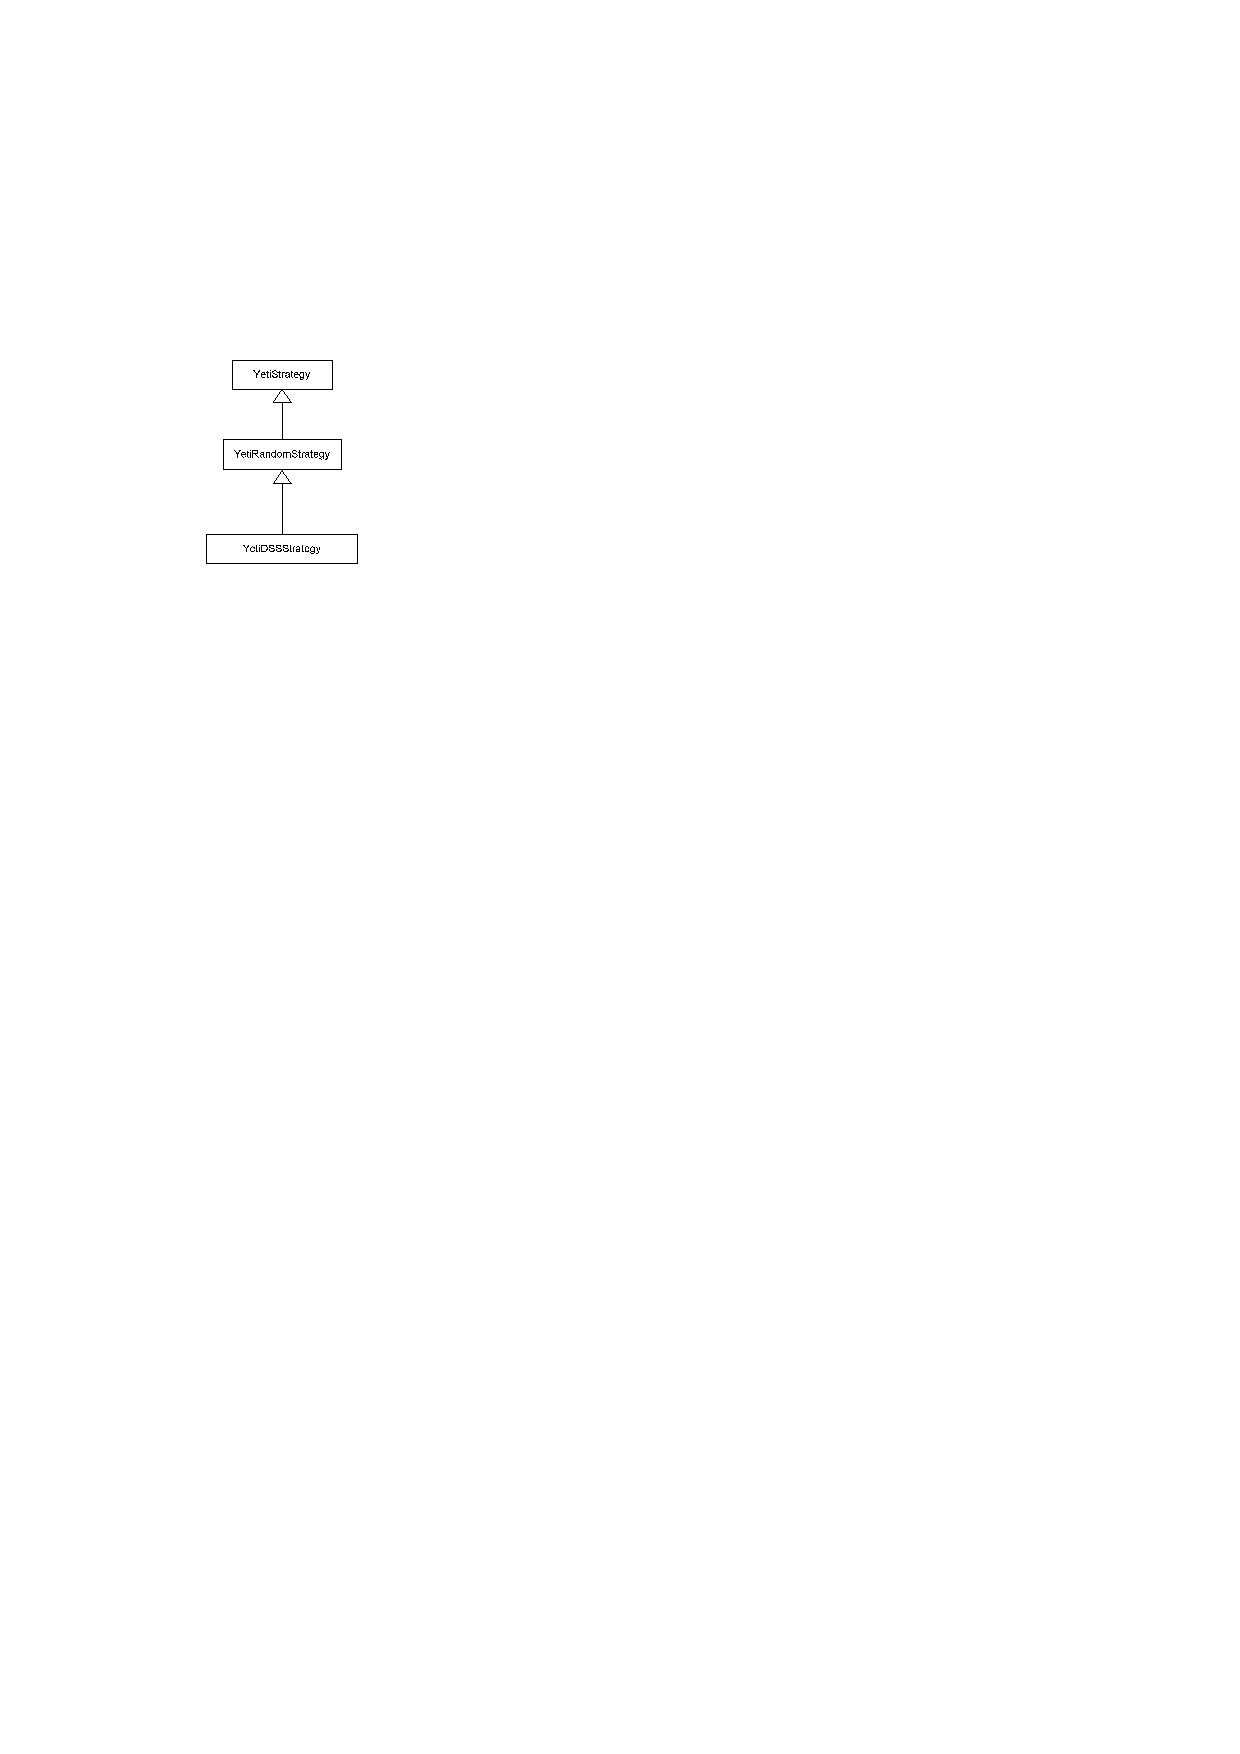
\includegraphics[width=4cm,height=5cm]{hierarchy.pdf}
\caption{Class Hierarchy of DSSR in YETI}
\label{fig:hierarchyofDSSR}
\end{figure}


If no particular strategy is defined during test initialisation then YETI will use its default random plus strategy in which the user can control the probability of null values and the percentage of newly created objects. Both probabilities are set to 10\% by default. \\
\indent YETI also provide an interactive Graphical User Interface (GUI) where a user can see the progress of the current test in real time. Besides GUI, YETI also provides extensive logs of the test session which are very helpful in fault tracking. For more details about YETI see references \cite{Oriol2010a} and \cite{Oriol2010}.

%%%%%%%%%%%%%%%%%    EVALUATION   %%%%%%%%%%%%%%%%%%%%


\section{Evaluation}
\subsection{Use of Qualitas Corpus for Evaluation}
To evaluate the performance of DSSR strategy we performed extensive testing of programs that cover full set of Java applications. Qualitas corpus \cite{Tempero2010a} is a curated collection of such open source java projects built with the aim to help testers in empirical research. These projects are collected in an organised form containing both the source and binary form. The reason for including source code is that most of the binaries do not include infrastructure code like code for demonstrating aspects of the system, testing, installation and building or management tasks. In its latest version 20101126, it contain 106 open source java projects. It is available in two distributions. The release version ``r'' and the evolution version ``e''. The release version is compact size which contain only the recent version of the projects while the evolution version is more detailed which consists of more than 10 different versions of each project.\\

\subsection{Evaluation by comparison under identical conditions}
To get a clear view of DSSR performance we determined the comparative performance of DSSR strategy with pure random strategy and random plus strategy by applying them to similar systems under identical conditions. Both the general factors like system software, hardware and YETI specific factors like percentage of null values, percentage of newly created objects and Interesting value injection probability were  kept constant for each test strategy. For all our experiments where applicable the interesting value injection probability was set to 0.5, which means that 50\% of the test values will be selected from the list of interesting values while remaining 50\% of the values will be selected randomly.\\

\subsection{Minimising the effect of Randomness}
\indent Random testing is probably the only strategy whose not only input is random but its output is also random. It is not necessary that all the faults it found in one test run can also be found in the second test run. Therefore the performance of random strategy cannot be evaluated from a few test sessions. To avoid the random behaviour of random testing every class was tested at least 30 times each by pure random, random plus and DSSR strategy. This is achieved by creating a batch executable script with the handy feature of YETI called compact report that logs each test report to a file for later evaluation.

\subsection{Performance measurement criteria}
Various measures including F-measure, P-measure and E-measure have been used by researchers to find the effectiveness of the random test strategy. E-measure (Expected number of failures detected) and P-measure (Probability of detecting at least one failure) received criticism from researchers \cite{Chen2008} and are not considered effective techniques for measuring efficiency of test strategy. F-measure (Number of test cases used to find the first fault) used by researchers  \cite{Chen1996}, \cite{Chen2004} is quite well known and initially we used it in our experiments to calculate the efficiency. After a few experiments we came to know that this was not the right choice because in some experiments the first strategy found first fault quickly than the second strategy but after the complete test session the first strategy found lower number of total faults than the second strategy. In our view it is not fair to prefer a strategy only because it found the first fault better without giving due consideration to the total number of faults. Moreover, for random testing F-measure is quite unpredictable because its value can be easily increased by adding more narrow conditional statements in the SUT. For example in the following program it is difficult for random testing to generate the exact number (3.3338) quickly and therefore the F-measure will be high.\\*

\begingroup
    \fontsize{7pt}{8pt}\selectfont
\noindent
\{ \\*
\indent if ( (value $>$  3.3337) \&\& (value $<$ 3.3339) )\\*
\indent \{ 10/0 \} \\* 
\} \\*
\endgroup
  
From the literature we also found that F-measure is used where testing stops after identification of first fault and the system is given back to the developers to remove the found bug where it make though not for random testing but since now automated random testing tests the whole system and print all of the faults found therefore F-measure is not the favourable choice. Therefore in all our experiments performance of the strategy was measured in terms of finding maximum number of faults in a particular number of test calls  \cite{Ciupa2007}, \cite{Pacheco2007a}, \cite{Ciupa2008b} which in our case was set to 10,0000 calls per class. This measurement was found effective because it clearly measured the performance of the strategy when all the other factors were kept constant.

\subsection{Experiments}
\indent Extensive experiments were carried out to evaluate the performance of DSSR strategy. Every class was tested 30 times by random, random plus and DSSR strategy. The total number of experiments performed are 100 x 30 x 30 x 30 = 9000. Each class was evaluated by 1 lac test cases in each experiment so The total number of test cases in 9000 experiments are  9000 x 1000000 = 9000000000. The automated oracle used for all experiments was the defined exception of the language because of the absence of the contracts and assertions in the code under test.\\
\indent Commands for executing the experiments using pure random, random plus and DSSR strategies are as follows. Here Prog1 is the name of the class and nTests is the number of tests set to be executed during this experiment.\\

\begingroup
    \fontsize{7pt}{10pt}\selectfont
\begin{itemize}
\item java yeti.Yeti -java -testModules=Prog1 -nTests=10000 -nologs -gui -random.
\item java yeti.Yeti -java -testModules=Prog1 -nTests=10000 -nologs -gui -randomPlus.
\item java yeti.Yeti -java -testModules=Prog1 -nTests=10000 -nologs -gui -DSSR.\\
\end{itemize}
\endgroup



All tests were performed using 64-bit Mac OS X Version 10.7.4 running on Intel(R) Core(TM)2 Duo CPU E8400 @ 3.00GHz with 6.00 GB RAM. Furthermore, Java(SE) Runtime Environment [Version 6.1.7601] was used. It took 4 days (96 hours) for this machine to process all the experiments.\\


%%%%%%%%%%%%%%%%%    RESULTS   %%%%%%%%%%%%%%%%%%%%

\section{Results}

Experimental finding indicate that in 10\% cases DSSR strategy performs better than pure random and random plus strategy, in 2\% of cases pure random performs better, in 50\% cases DSSR and random plus are equivalent and in 38\% random plus performs better. 


\begin{table} [ht]
\caption{Summary of the total 9000 experiments }
\center
\begin{tabular} {|c|c|c|c|c|c|}
\hline\hline
Strategy Name & Mean & Median & Standard Deviation & Min & Max \\[1ex]
\hline
Random  &   &  &  &  & \\
Random Plus  &   &  &  &  & \\
DSSR &  &  &  &  & \\
\hline
\end{tabular}
\label{table:TestResults}
\end{table}

From the above table we can see that DSSR has the highest Mean value of finding faults which means that DSSR performs better then random and Random plus. The reason for small improvement instead of 10 and 20\% is described in detail in Discussion section. Similarly the other noticeable improvement is the minimum number of faults DSSR can find is 376 while for random and random plus it is 340 and 344 respectively which means that DSSR strategy always find some of the faults which random and random plus might not. On the other hand DSSR finds maximum 574 faults versus 579 faults of random and random plus but this difference is very small and can be ignored. During the experiments we also found that in some classes like AntClassLoader (Ant project),  Server (Freecs project), BaseFont (itext project) and Util (JsXe project) DSSR strategy found higher number of minimum and maximum faults where as in the same classes random and random plus found 0 or very few faults.  \\

\begin{comment}
\begin{figure}[ht]
\centering
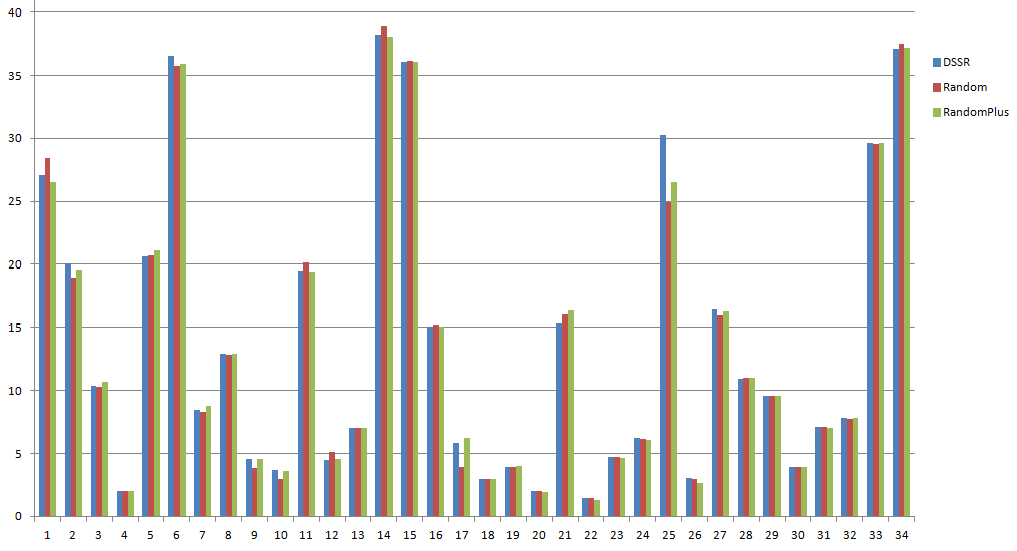
\includegraphics[width=9cm,height=7cm]{newResults.png}
\caption{Test Results of 34 classes from 16 Java projects.}
\label{fig:Result1}
\end{figure}
\end{comment}


Figure \ref{fig:Result1} show the results of each experiments using bar chart. From the figure we can see that in few of the cases all the three strategies found equal number of faults while in most cases if not all DSSR performs better than random and random plus strategy.


%%%%%%%%%%%%%%%%%    DISCUSSION   %%%%%%%%%%%%%%%%%%%%

\section{Discussion}
\textbf{Performance of DSSR strategy, Random strategy and Random plus strategy in terms of finding faults:} 
Analysis of results revealed that DSSR performs better than random and random plus in programs with block and strip pattern of faults. However, since not all the programs contain faults in the form of block and strip patterns therefore the results do not show a significant performance change. \\
\indent \textbf{Time taken by DSSR strategy, Random strategy and Random plus strategy to execute tests:}
To execute equal number of test cases, DSSR strategy took slightly more execution time than pure random and random plus test strategy. It is not unusual and we were expecting similar behaviour because pure random algorithm selects random input of the required type with minimum calculation and therefore its process is very quick. On the other hand random plus and DSSR strategy performs additional computation when it maintains the list of interesting values and selects the correct type test values from the list when required. The desired process of adding values to the list and selecting the required values from the list consumes extra time which is the main reason that DSSR strategy takes a little extra time. Thus in executing tests random strategy, random plus and DSSR strategy comes first, second and third respectively. \\
\indent \textbf{Effect of test duration in terms of time and number of tests on test results:} 
We found that test duration increases either because of  increase in time or number of test cases which results in improving the performance of DSSR strategy than random and random plus. It is because when test duration or number of tests increases, the list of interesting values also increases and in turn DSSR strategy get enough relevant values in the list of interesting values and can easily pick one from the list instead of selecting it randomly or from static list of random plus.\\
\indent \textbf{Effect of number of faults on results:} 
We also found that DSSR strategy performs better when the number of faults are more in the code. The reason is that when a fault is found in the code, DSSR strategy adds the neighbouring values of the fault finding value to the list of interesting values. Doing this increases the list of interesting values and the strategy is provided with more relevant test data resulting in higher chance of finding faults.\\
\indent \textbf{Can Pure Random and Random Plus Testing perform better than DSSR strategy:}
The experimental results indicated that pure random and random plus testing can perform better than DSSR strategy if the SUT contain point pattern of failures rather than block and strip pattern. It is due to the fact that in such cases faults don't lay in the neighbourhood of found fault and adding neighbouring values of the founded fault dont make any impact on performance therefore the extra computational time becomes a liability.\\
\indent \textbf{DSSR strategy Dependance on Random and Random Plus Testing:}
During the experiments we found that if the fault finding value is not in the list of interesting values then the test is dependant on random testing. In that case DSSR strategy has to wait for random testing to find the first fault and only then DSSR strategy will add its neighbouring values to the list of interesting values.


%%%%%%%%%%%%%%%%%    CONCLUSION   %%%%%%%%%%%%%%%%%%%%


\section{Conclusion}
The main goal of the present study was to develop a new random strategy which could find more faults in lower number of test cases and shorter execution time. The experimental findings revealed that DSSR strategy was up to 20\% more effective in finding faults as compared to random strategy and up to 10 \% more effective than random plus strategy. The DSSR strategy not only gave more consistent results but it proved more effective in terms of detecting faults as compared to random and random plus testing.\\
\indent Improvement in performance of DSSR strategy over random strategy was achieved by taking advantage of Random Plus and fault neighbouring values. Random plus incorporated not only border values but it also added values having higher chances of finding faults in the SUT to the list of interesting values.\\
\indent The DSSR strategy is highly effective in case of systems containing block and strip pattern of failure across the input domain.\\
\indent Due to the additional steps of scanning the list of interesting values for better test values and addition of fault finding test value and its neighbour values, the DSSR strategy takes up to 5\% more time to execute equal number of test cases than pure random and random plus. \\
\indent In the current version of DSSR strategy, it might depend on random or random plus strategy for finding the first fault if the fault test value was not in the list of interesting values. Once the first fault is found only then DSSR strategy could make an impact on the performance of test strategy.\\
\indent The limitation of random plus strategy is that it maintains a static list of interesting values which remains the same for each program under test, and can be effective in many cases but not always. The better approach will be to have a dynamic list of interesting values that is automatically updated for every program which can be achieved by adding the program literals and its surrounding values to the list of interesting values prior to starting every new test session.


%%%%%%%%%%%%%%%%%    FUTURE WORK   %%%%%%%%%%%%%%%%%%%%



\section{Future Work}
From the research we came to know that random testing is not very good in generating a test value when the scope of a variable is too narrow as in the following example.  \\
\begingroup
    \fontsize{7pt}{10pt}\selectfont
\noindent
\{ \\*   
\indent if(value == 34.4445) \\*
\indent \{ 10/0 \} \\* 
\} \\*
\endgroup
\indent We also know that if the fault finding value is not in the list than DSSR has to wait for random testing to generate the fault finding value and only after that DSSR strategy will add that value and its surrounding values to the list of interesting values. To decrease the dependancy of DSSR strategy on random and random plus strategy, further work is in progress to add constant literals from the SUT to the list of interesting values in a dynamic fashion. These literals can be obtained either from .java or .class files of the SUT. We are also working to add  neighbouring values of the literals to the list of interesting values. \\
\indent Thus if we have the above example then the value 34.4445 and its surrounding values will be added to the list of interesting values before the test starts and DSSR strategy will no more be dependent on random testing to find the first fault. Finally, it will also be interesting to evaluate the DSSR strategy in terms of coverage because the newly added values are most suitable for test cases and therefore can increase branch coverage. 

\bibliographystyle{IEEEtran}
\bibliography{bare_conf}

\end{document}


